\chapter{透镜与像}\label{ch:g8:lenses-images}

针孔相机以极高的代价换来了清晰的小像：
几乎没有光。然而你自己的眼睛
整天都在后壁上描绘出明亮清晰的世界，
却看不见任何针孔。眼睛的秘密在于一块弯曲的玻璃状物，
它能汇聚整束光线，并使之有序地弯折 --- 这便是透镜，
也是相机、眼镜、放大镜以及本章的主角。

\section{两类透镜}

\begin{definition}[凸透镜与凹透镜]\label{def:g8:lenses-images:families}
称\emph{透镜}\index{透镜}为一块透明材料，
--- 玻璃或透明塑料 --- 制成，表面弯曲，
（光射入玻璃时会发生折射，
而折射的精确规律留待高中分册学习）。
两类透镜如下：
\begin{enumerate}
  \item \emph{凸透镜}\index{凸透镜} ---
        中间比边缘厚 --- 使光束的
        光线\emph{相互靠拢}；
  \item \emph{凹透镜}\index{凹透镜} ---
        中间比边缘薄 --- 使光线分散开。
\end{enumerate}
用指尖划过一片眼镜片：中间鼓起还是中间凹陷，
便能把世上每一块透镜归入其所属的类别。
\end{definition}

\begin{definition}[焦点与焦距]\label{def:g8:lenses-images:focus}
让一束平行光 --- 比如阳光 --- 穿过凸透镜，
折射后的光线都相交于透镜后方的一点，
即\emph{焦点}\index{焦点}。从透镜到焦点的距离
称为\emph{焦距}\index{焦距}
$f$，即透镜特有的唯一特征数。
曲率大、较厚的透镜折光强 --- 焦距 $f$ 较短；
曲率小的透镜折光弱 --- 焦距 $f$ 较长。
\end{definition}

\begin{omfigure}
\begin{tikzpicture}[scale=0.8]
  \draw[thick, fill=blue!6]
    (2.6,-1.6) .. controls (3.3,0) .. (2.6,1.6)
    .. controls (1.9,0) .. (2.6,-1.6);
  \foreach \y in {-1.2,-0.6,0,0.6,1.2} {
    \draw[-Stealth, omThm, thick] (0.2,\y) -- (2.35,\y);
    \draw[omThm, thick] (2.35,\y) -- (5.6,0);
  }
  \fill[omDef] (5.6,0) circle (0.09);
  \node[below, font=\small] at (5.6,-0.25) {焦点};
  \draw[Stealth-Stealth, omExo] (2.6,-1.9) -- (5.6,-1.9);
  \node[below, font=\small, omExo] at (4.1,-2.0)
    {焦距 $f$};
  \begin{scope}[xshift=7.6cm]
    \draw[thick, fill=blue!6]
      (0.95,1.6) .. controls (1.25,0.55) and (1.25,-0.55) ..
      (0.95,-1.6) -- (1.65,-1.6)
      .. controls (1.35,-0.55) and (1.35,0.55) .. (1.65,1.6)
      -- cycle;
    \foreach \y in {-1.0,-0.5,0,0.5,1.0} {
      \draw[-Stealth, omThm, thick] (0,\y) -- (0.9,\y);
      \draw[omThm, thick] (0.9,\y) -- (1.3,\y) -- (3.6,{\y*1.9});
    }
    \node[below, font=\small] at (1.8,-2.0)
      {发散：光束散开};
  \end{scope}
\end{tikzpicture}

{\small 两类透镜的作用：凸透镜把一束平行光
会聚到焦点；凹透镜使光束
散开。}
\end{omfigure}

\begin{method}[测量焦距]\label{met:g8:lenses-images:measure}
对任一凸透镜，只需一分钟和一扇远处的窗户：
\begin{enumerate}
  \item 使墙面正对一个明亮的\emph{远处}景物 ---
        即窗户及窗外的世界；
  \item 将透镜靠近墙面，并缓慢向后移开，
        直到景物在墙上形成一幅小而清晰的
        像（倒立的 --- 这早在意料之中）；
  \item 测量透镜到墙面的距离：对远处景物，
        这一距离\emph{正是}焦距 ---
        远处光线几乎平行地到达，
        而平行光线会聚于焦点。
\end{enumerate}
放大镜的焦距约为 \qty{10}{cm}；眼镜片的焦距
为几十厘米；相机短粗的镜头则只有几厘米。
\end{method}

\begin{remark}[取火镜]\label{rem:g8:lenses-images:burning}
在凸透镜的焦点处，整束阳光的宽度
全部挤进一个炽热的光斑 --- 能量集中得
足以在数秒内烧焦纸张、引燃火苗。应当把它
视为其本来面目：袖珍版的太阳灶原理。
切勿将阳光聚焦于易燃物附近，切勿对准
皮肤或衣物 --- 还要再说一遍：切勿
\emph{透过}任何透镜直视太阳：眼睛自身的聚焦
加上透镜的聚焦，会瞬间造成无痛却永久的烧伤。
\end{remark}

\section{作为成像器件的透镜}

\begin{proposition}[实像]\label{prop:g8:lenses-images:realimage}
凸透镜将物体上每一点发出的光线
并把它们送到另一侧的对应点上：
逐点地组成一幅真实的图像 --- 即
\emph{实像}\index{实像} --- 可以用屏幕接收。
。像是倒立的，与针孔成像一样，但
更为明亮：每个点都能收集整块透镜上的光，
而针孔只透过一缕光线。几何上的经验规则是：
远处物体的像小，且靠近焦点；随着物体靠近透镜，
像向远处退去，
并逐渐变大。
\end{proposition}

\begin{omfigure}
\begin{tikzpicture}[scale=0.8]
  \draw[-Stealth, very thick, omDef] (0.8,0) -- (0.8,1.5);
  \node[left, font=\small] at (0.65,0.75) {物体};
  \draw[thick, fill=blue!6]
    (4.6,-2.0) .. controls (5.3,0) .. (4.6,2.0)
    .. controls (3.9,0) .. (4.6,-2.0);
  \draw[dashed] (0,0) -- (10.6,0);
  \draw[omThm, thick] (0.8,1.5) -- (4.6,1.5) -- (8.9,-1.13);
  \draw[omThm, thick] (0.8,1.5) -- (8.9,-1.13);
  \fill[omDef] (6.05,0) circle (0.07);
  \node[below, font=\footnotesize] at (6.05,-0.15) {焦点};
  \draw[-Stealth, very thick, omDef] (8.9,0) -- (8.9,-1.13);
  \node[right, font=\small] at (9.05,-0.6)
    {实像：倒立，可承接};
\end{tikzpicture}

{\small 成像：物体顶端发出的光线——一条过透镜中心，
一条经透镜折向焦点——
在另一侧再次相交，图像在那里合成，
倒立。}
\end{omfigure}

\begin{example}[相机与眼睛：同一种结构]\label{ex:g8:lenses-images:cameraeye}
相机就是装在箱子里的成像器：前面是凸透镜，
后面是感光屏，像倒立地成在屏上
（软件会替你把文件转正）。你的眼睛是同一台机器，只不过长在活体中：
凸透镜位于瞳孔之后，
\emph{视网膜}充当后方的屏幕，像同样倒立——
大脑会把它翻过来，这一点在针孔成像时已经讲过。
对焦则各有妙处：相机移动
镜头；眼睛里那块柔软的晶状体\emph{改变形状}，
看近处时鼓起变厚，看远处时松弛变薄——
不妨感受一下连续读书一小时后的用力。
\end{example}

\begin{example}[眼镜]\label{ex:g8:lenses-images:spectacles}
眼睛自身的调节不足时，
便在前面加一块透镜予以补充。近视眼的会聚能力过强——
远处景物的像\emph{在视网膜之前}便已会聚，
以致模糊。此时需要一片\emph{凹透镜}，使光线略微散开，
远视眼（以及大多数上了年纪的人）的会聚能力偏弱，
看近处时不够用：此时需要\emph{凸透镜}补足所缺的
会聚能力——老花镜正是这样朴实的小透镜，
与放大镜是近亲。透镜分两类，
模糊亦分两类。
\end{example}

\section{放大镜}

\begin{omfigure}
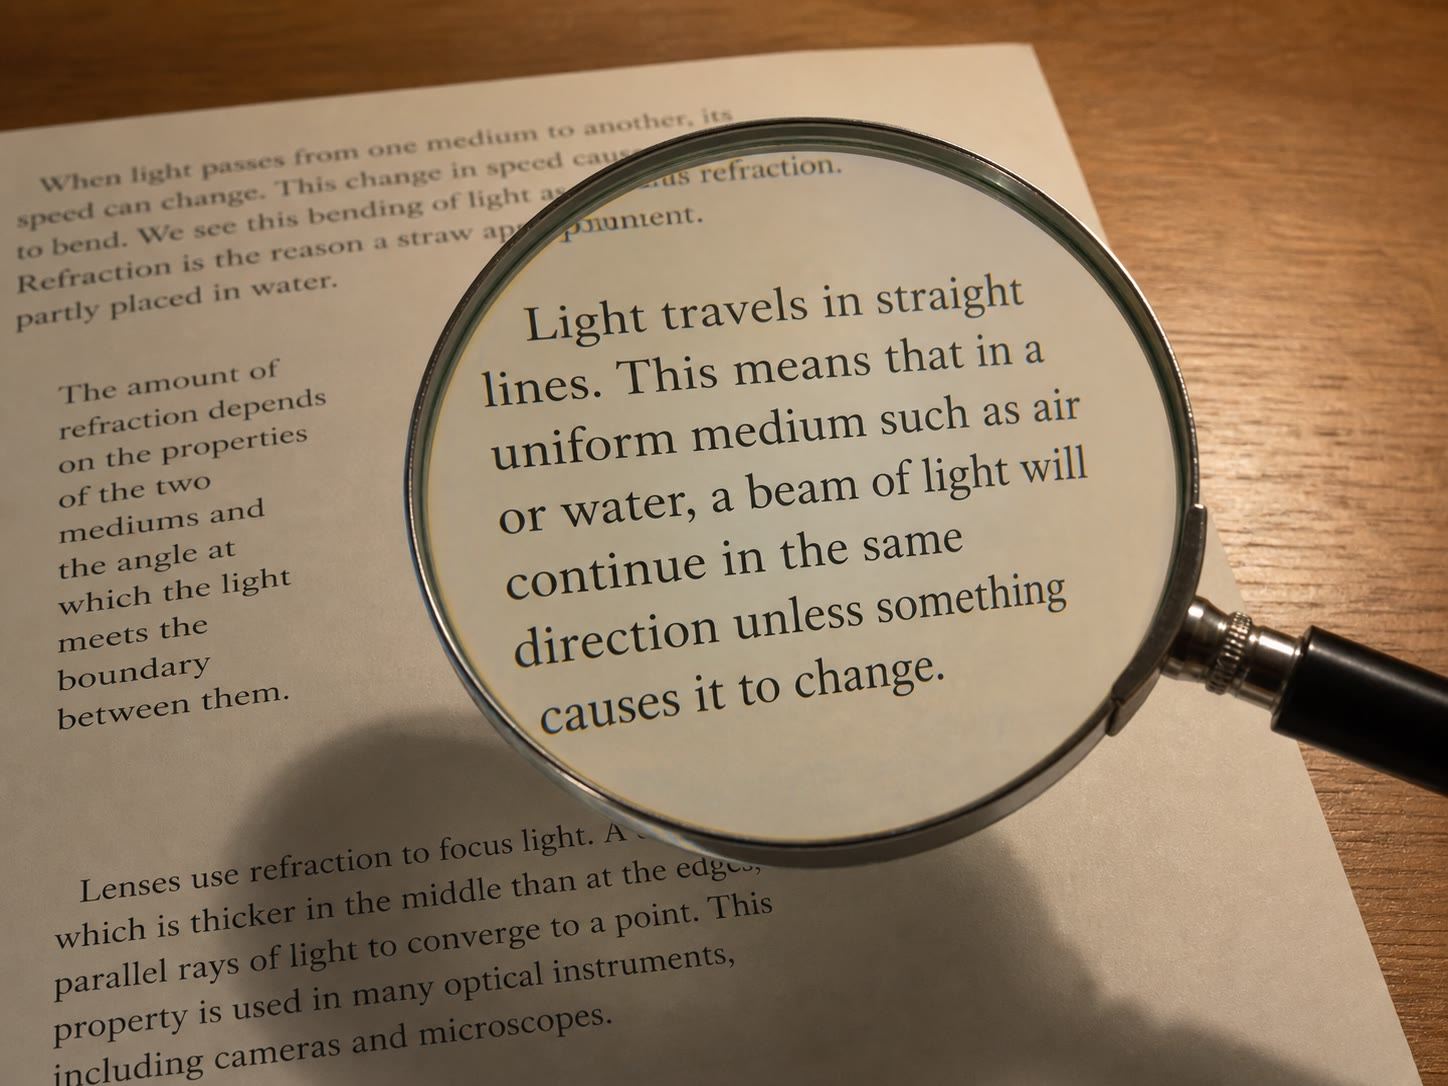
\includegraphics[width=0.5\linewidth]{images/book1/ai/g8-lenses-magnifier.jpg}

{\small 放大镜工作示意：透镜置于比焦距更近的位置时，所见文字正立且被放大。}
\end{omfigure}

\begin{example}[焦距之内]\label{ex:g8:lenses-images:magnifier}
将凸透镜\emph{靠近}邮票，使二者距离小于焦距，
图像的性质随之改变：不再有像落在
任何屏幕上；透过透镜看去，你看到的是
正立、原位且放大的邮票。透镜使
邮票发出的光线进入眼睛时，\emph{仿佛}来自
镜后一枚更大的邮票——这是一种量身定制的幻象，
与镜子中的幻象世界是近亲。钟表匠、集邮者，
以及童年时拿着放大镜的你自己，
都曾用过它；这一戏法的完整光线几何，
是高中分册中的一颗明珠。
\end{example}

\begin{remark}[层层叠加的仪器]\label{rem:g8:lenses-images:instruments}
把透镜叠加起来，世界便为之打开。两块凸透镜可组成
显微镜：第一块形成液滴的大实像，
第二块再将该像放大——分子学说的捍卫者由此获得了
第一批直接的盟友。大透镜（或曲面镜）
加上放大镜，便成望远镜：遥远星系的
微弱平行光被汇聚成实像，再被放大
送入惊叹的眼睛。人类文明中的每一种光学仪器，
都是本章两个想法的各种组合：先汇聚，再放大——
只是排列方式各不相同。
\end{remark}

\section{练习}

\begin{exercise}[$\star$]\label{exo:g8:lenses-images:1}
用触觉分辨：指尖如何区分凸透镜与
凹透镜？它们各自对平行光束有何作用？
\end{exercise}

\begin{exercise}[$\star$]\label{exo:g8:lenses-images:2}
给出焦点与焦距的定义。焦距较短说明透镜的
曲率与偏折光线的能力有何特点？
\end{exercise}

\begin{exercise}[$\star$]\label{exo:g8:lenses-images:3}
描述用窗户与墙面测量 $f$ 的方法。为什么
所看的景物必须距离很远？
\end{exercise}

\begin{exercise}[$\star$]\label{exo:g8:lenses-images:4}
说明取火透镜的两条安全规则，
并说明各条规则存在的原因。
\end{exercise}

\begin{exercise}[$\star$]\label{exo:g8:lenses-images:5}
什么是实像？给出实像的两个标志性性质，
以及透镜相对针孔的优点。
\end{exercise}

\begin{exercise}[$\star$]\label{exo:g8:lenses-images:6}
将相机与眼睛对应起来：两者中，什么分别充当透镜、
屏幕和对焦机构？
\end{exercise}

\begin{exercise}[$\star$]\label{exo:g8:lenses-images:7}
哪一类眼镜适合近视眼，为什么？
老花眼又该配哪一类？
\end{exercise}

\begin{exercise}[$\star$]\label{exo:g8:lenses-images:8}
在放大镜的小把戏中，邮票的位置须满足
什么条件？此时眼睛所看到的是
哪一种“像”？
\end{exercise}

\begin{exercise}[$\star\star$]\label{exo:g8:lenses-images:9}
一位摄影师的拍摄对象正朝相机走来。
按经验法则，为使像在感光元件上保持清晰，
镜头应朝哪个方向移动？人眼在同样情况下
又是怎样做的？
\end{exercise}

\begin{exercise}[$\star\star$]\label{exo:g8:lenses-images:10}
晴天里，随手放在干树叶上的透镜就是一处
潜在的火源，但只有在透镜到树叶的某一特定距离时
才会如此。是哪一个距离？为什么恰好是
这个距离？
\end{exercise}

\begin{exercise}[$\star\star$]\label{exo:g8:lenses-images:11}
爷爷的老花镜既能充当应急放大镜，
节假日里还可用来聚光点烟——
而近视的孙子所戴的眼镜两样都做不到。
请解释这两件家事。
\end{exercise}

\begin{exercise}[$\star\star\star$]\label{exo:g8:lenses-images:12}
显微镜与望远镜都由两块凸透镜组成，
但一个用来放大液滴，另一个用来观测星系。
请对比两者的两个阶段：在两种仪器中，第一块透镜
分别接收并产生什么（近处物体与几乎平行的星光相比），
以及为什么望远镜的第一块透镜尤其要\emph{大}，
而显微镜的第一块透镜则要求
\emph{曲率很大}？
\end{exercise}

=\section{周末问题：验光师的工作台}

=\begin{problem}[{周末问题 --- 在镇上的验光店当学徒：焦距、配镜
与一架裂了的望远镜}]
=\label{pb:g8:lenses-images:1}
验光店的一天：要分拣的镜片、要配对的眼镜，
以及一位顾客已拆成零件的望远镜。

=\medskip\noindent\textbf{第一部分 --- 整理托盘。}
一个抽屉翻倒，把存货混在了一起。
=\begin{enumerate}
  \item 请提出两种快速检验方法：一种用手摸，另一种借助
        窗户与墙壁，用以区分凸透镜与
        凹透镜。
  \item 透镜 A 将街道的清晰像投射到墙上，
        墙面距透镜 \qty{25}{cm}。其焦距与类别如何？
  \item 透镜 B 在墙上任何距离处都成不了像，
        透过它看到的物体都变小了。
        它属于哪一类？
  \item 透镜 C 与 D 均为凸透镜；C 使窗外景物成像，
        像位于 \qty{10}{cm} 处，D 的像位于 \qty{40}{cm} 处。
        哪一块透镜的曲率更大、
        折光能力更强？
=\end{enumerate}

=\medskip\noindent\textbf{第二部分 --- 配镜。}
=\begin{enumerate}[resume]
  \item 一位顾客看远处的路标模糊，但读菜单
        毫不费力。请诊断其眼睛的问题，并开出
        应配的眼镜类型。
  \item 另一位顾客把报纸拿在臂长处阅读，并抱怨
        自己的胳膊“太短了”。请诊断，并开出
        相应的眼镜。
  \item 验光师提醒这位顾客：“你的新
        老花镜会让远山变得模糊。”为什么
        老花镜只适用于近处的书页？
  \item 一个小孩问，为什么验光师的试戴镜片会使
        视力表晃动，而他自己的眼睛却
        “很好”。矫正镜片会
        对一只对焦良好的眼睛产生什么作用？
=\end{enumerate}

=\medskip\noindent\textbf{第三部分 --- 破损的
=望远镜。}
一位顾客带来一架观星望远镜，其物镜
已经破裂，问盒中的备用放大镜能否
代替它。
=\begin{enumerate}[resume]
  \item 请说出完好的望远镜中两块透镜各自的作用：
        大物镜从恒星接收什么，
        并将其会聚成像；小目镜对此
        又做了什么？
  \item 物镜大如碟子，目镜小如硬币。
        为什么物镜的\emph{口径}对观测暗弱恒星
        如此重要？
  \item 备用放大镜的曲率很大，但只有
        硬币大小。请评价这一替换：在仪器前端
        会得到什么、又会失去什么？
  \item 最后，请以验光师的一句话箴言收束全天，
        箴言涉及货架上每件仪器——眼镜、放大镜、
        照相机、望远镜——并用两个动词概括
        透镜为文明所做的事。
=\end{enumerate}
=\end{problem}
